\begin{question}
\noindent As part of a space research project, two research drones, $P$ and $Q$, are launched simultaneously from a base station $B$ on a remote desert test site to record atmospheric data.

\begin{itemize}
    \item Drone $P$ flies on a bearing of $050^\circ$ from $B$ and travels a distance of $12$ km before hovering.
    \item Drone $Q$ flies on a bearing of $140^\circ$ from $B$ and travels a distance of $9$ km before hovering.
\end{itemize}

\begin{center}
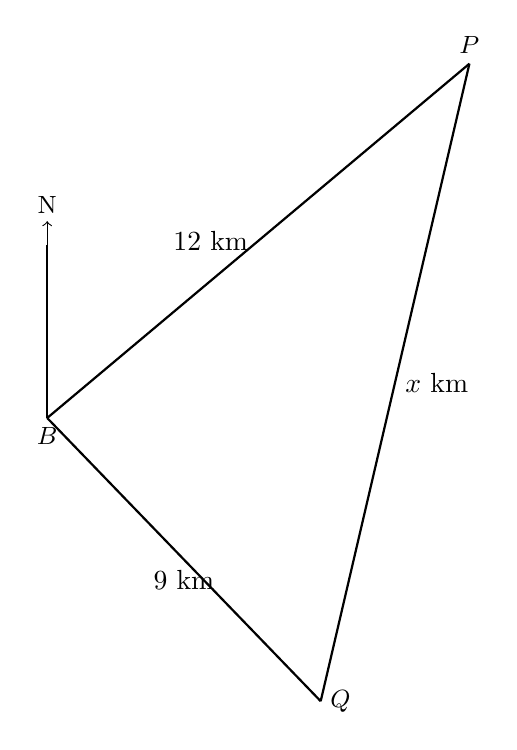
\begin{tikzpicture}[scale=1, transform shape]
    \coordinate (B) at (0,0);
    %bearing of P is 50 therefore angle made with horizontal will be 90-50 =40
    \coordinate (P) at (40:7);
    %bearing of Q from vertical is 140, therefore angle with horizontal will be 90-140 = -50. Going with 46 degrees to the right angle less obvious
    \coordinate (Q) at (-46:5);

    % North line at B
    \draw[thick] (B) -- (0,2.2);
    \draw[->] (0,2.2) -- (0,2.5);
    \node at (0,2.7) [font=\small] {N};

    % Draw the triangle sides
    \draw[thick] (B) -- (P) node[midway, left] {$12$ km};
    \draw[thick] (B) -- (Q) node[midway, below] {$9$ km};
    \draw[thick] (P) -- (Q) node[midway, right] {$x$ km};

    % Labels
    \node at (B) [below,font=\small] {$B$};
    \node at (P) [above,font=\small] {$P$};
    \node at (Q) [right,font=\small] {$Q$};

\end{tikzpicture}
\end{center}

\noindent Calculate the distance $PQ$ between the two drones, giving your answer to 3 significant figures.

\vspace{5cm}

\begin{flushright}
\answerunit{$\text{km}$}{4}
\end{flushright}
\end{question}